\documentclass[journal]{IEEEtran}
\usepackage{graphicx}
\usepackage[scriptsize]{caption}
\renewcommand{\arraystretch}{1.1}

\begin{document}

\newcommand{\labtitlegen}{
    \twocolumn[{
    \begin{center}
        \LARGE\labtitle \\ \bigskip \large\name \\ \bigskip
        \labsection \\ 
        \textbf{TA} \\ \taname \\% \bigskip \textbf{Lab Partners} \\
%        \partnername
    \end{center}
    }]
}

%% Change these variables
\newcommand{\labtitle}{Experiment 3: Magnetism}
\newcommand{\name}{604-296-523}
\newcommand{\labsection}{Section 2, Wednesday 8AM}
\newcommand{\labdate}{February 11, 2015}
\newcommand{\taname}{Elwin Martin}
\newcommand{\partnername}{Kari Kawashima}


%% This creates your lab cover page.
\labtitlegen

\newcommand{\mval}[3]{$#1 \pm #2 #3$}

\section{Introduction}

Steady state sources generate particular kinds of magnetic fields - often with
high degrees of symmetry, and existing only in enclosed regions or falling off
as the cube of the distance.

In this paper two types of fields will be explored - those of a torroidal
solenoid, and those of a permanent magnet. This will be done using both a hall
probe and a simple scale. The former will measure the magnetic field magnitude
directly, and the latter can measure repulsive forces of interacting magnets.

In addition, it will be verified whether induced current between two mutual
inductors is fully explained by Faraday's law.
\section{Results}

A torroidal solenoid with $N=100$ turns was powered with a voltage of $11.92
\pm 0.005 V$. Measured with a multimeter, the entire solenoid had a resistance
of $11.0 \pm 0.05 \Omega$. The inner radius in which the coils pass is 3.2 cm,
and the outer radius is 18cm. Measurements were taken of the azimuthal magnetic
field, starting at the innermost point, with the hall probe almost directly in
contact with the inner edge of the coils, and every $0.5 cm$ radially outward.
The measurements are shown in Figure~\ref{fig:toroid_hall}.

\begin{figure}[ht!]
\centering
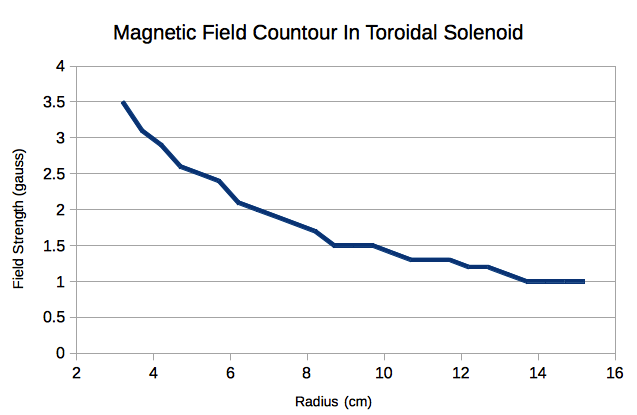
\includegraphics[width=80mm]{toroid_hall.png}
\caption{Measurement of azimuthal magnetic field
magnitude in solenoid.}
\label{fig:toroid_hall}
\end{figure}


Measurements inside the inner radius and outside the outer radius were either 0
or close to it - they were within the natural noise of the Hall sensor. It was
also verified that measurements taken at various heights and various radial
angles (moving the hall probe vertically and horizontally, keeping the radius
the same) did not effect the measured magnetic field.

The same Hall sensor was used to measure the z-component of the magnetic field
of a permanent magnet under two types of displacement. The magnet was oriented
vertically, such that the north side was pointing upward. Measurements were
first taken from directly above the magnet, starting from a point $2.8 cm$ away
from the center ($1.5 cm$ above the surface). The measurements are shown in
Figure~\ref{fig:maghall_vert}.

\begin{figure}[ht!]
\centering
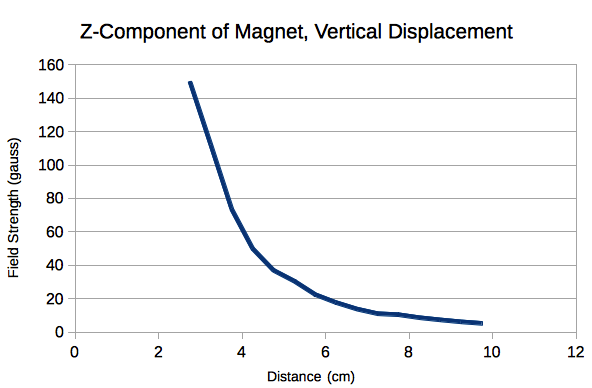
\includegraphics[width=80mm]{maghall_vert.png}
\caption{Measurement of z-component of magnetic field above a permanent magnet,
as a function of vertical distance from the center.}
\label{fig:maghall_vert}
\end{figure}

Similar measurements were taken with horizontal displacement. The hall sensor
was placed near the vertical center of the magnetic, aligned with the
z-component of the magnetic field, and gradually moved away. The initial
distance was $3.2 cm$ ($2.1 cm$ from the surface). The measurements are shown
in Figure~\ref{fig:maghall_horiz}.

\begin{figure}[ht!]
\centering
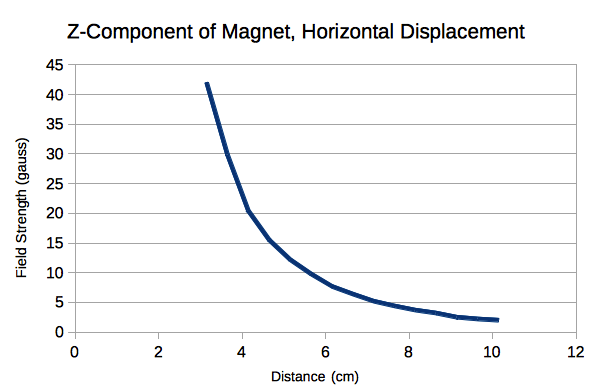
\includegraphics[width=80mm]{maghall_horiz.png}
\caption{Measurement of z-component of magnetic field near a permanent magnet,
as a function of the horizontal distance to the center.}
\label{fig:maghall_horiz}
\end{figure}

The dimensions of the magnet used in both measurements (same magnet was used)
was $2.1x2.5 cm$.

A nearly identical magnet was used to measure the force between two dipole
permanent magnets as a function of the distance between them. The measurements
were taken as follows.

One magnet was placed on a scale, and weighed without the influence of the
other magnet. Its weight was found to be $47.1 g$. Then the other magnet was
placed above it on a sliding track with measurements on it, used to measure the
center-to-center distance between the two magnets. They were oriented such that
the force between them was repulsive, meaning that the measurement of the scale
grew as the two magnets were moved closer together.

The data, with initial weight subtracted out (so that only the repulsive force
remains), is shown in Figure~\ref{fig:magforce}. Force is measured in
grams, since only the analysis will only be looking for the proportionality of
the distance and the force, and any extra constants (e.g. multiplying by g)
would be ignored.

\begin{figure}[ht!]
\centering
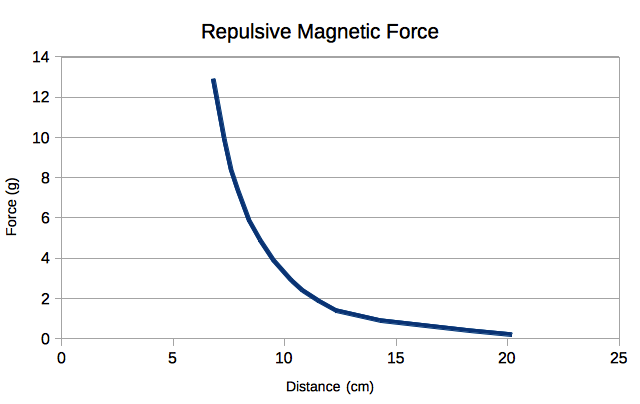
\includegraphics[width=80mm]{magforce.png}
\caption{Measurement of the repulsive force between two magnets, as a function
of center-to-center distance between them.}
\label{fig:magforce}
\end{figure}

It is further possible to observe the effects of a magnetic field on induced
current. To observe this, two solenoids were used, one placed inside of the
other, such that they had a strong mutual inductance. The outer coil has 100
turns, and the inner coil has $n=8 turns/mm$ and a diameter of $2.2 cm$. The
inner current is varied sinusoidally. Current is measured through a series
resistor of $12.1 \Omega$, by measuring the voltage across it on CH 0. The
voltage induced in the outer coil is measured on CH 1. The layout is shown in
Figure~\ref{fig:ac_circuit}.

\begin{figure}[ht!]
\centering
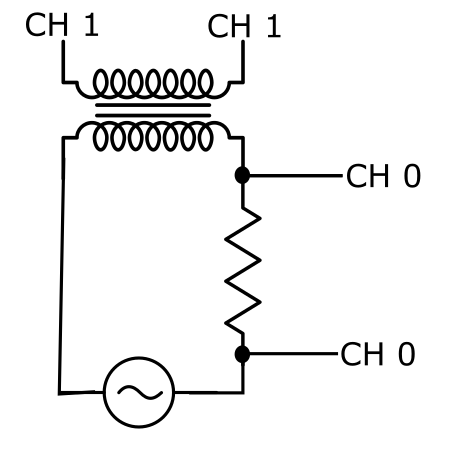
\includegraphics[width=40mm]{circuit.png}
\caption{The circuit used to measure induced current in a coil. The resistor is
$12.1 \Omega$, and used to measure current over Ch 0.}
\label{fig:ac_circuit}
\end{figure}

This allows measurement both of the current creating a magnetic flux, and the
voltage that that magnetic flux induces. It is shows in
Figure~\ref{fig:ac_induced}.

\begin{figure}[ht!]
\centering
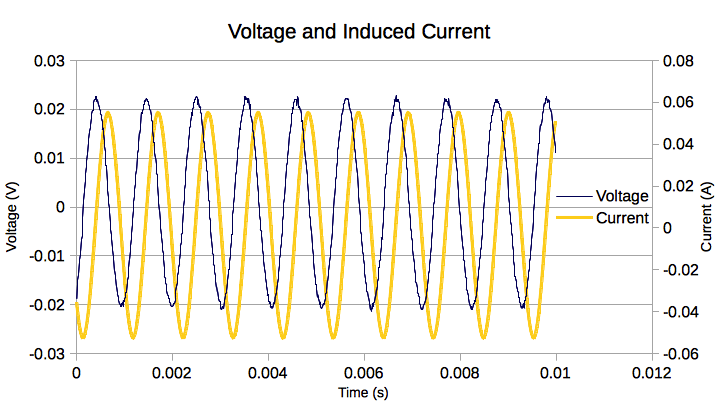
\includegraphics[width=80mm]{ac_induced.png}
\caption{Voltage induced between coils with a mutual inductance, and current in
the primary coil.}
\label{fig:ac_induced}
\end{figure}

\section{Analysis}

In addition to the standard results of a linear regression - the slope and
intercept, with corresponding uncertainties - the correlation coefficient
(Equation~\ref{corr}) will be used to get a better picture of how well the
measured data fits the models.

\begin{equation}
\label{corr}
r = \frac{\sum (x_i - \bar x)(y_i - \bar y)}{\sqrt{\sum (x_i - \bar x)^2
\sum(y_i - \bar y)^2}}
\end{equation}

This value describes how well the linear model fits the given data - or,
alternatively, how well the line given by the linear regression can predict the
data.

The toroid has a magnetic field that imitates the field shape of an infinite
line current. According to Ampere's law, the magnetic field around a current
should follow the relation \ref{ampere}.

\begin{equation}
\label{ampere}
\oint_C {Bd\ell = \mu _0 I_C }
\end{equation}

At a distance of r from the current source, the left-hand side can be
integrated using symmetry (it is a constant azimuthal magnetic field), and the
right hand side remains the same.

\begin{displaymath}
B(r) 2 \pi r = \mu _0 I_C
\end{displaymath}

Meaning that the magnetic field magnitude itself follows the relation

\begin{displaymath}
B(r) = \frac{\mu _0 I_C}{2 \pi r}
\end{displaymath}

This law is followed very closely in a toroidal solenoid - the proportionality
is the same, and the containment of the flux means the magnetic field does not
decay slower inside the solenoid, but the current flowing through the center of
the solenoid is proportional to both the current in the wire and the number of
turns N. The full law is given by Equation~\ref{b_sol}.

\begin{equation}
\label{b_sol}
B(r) = \frac{\mu _0 N I_C}{2 \pi r}
\end{equation}

This is supported by the fact that measurements did not change upon changing
the height or location of the Hall meter, as long as the radial distance
remained the same. This means that the magnetic field magnitude is a function
of the radius only.

Taking the data shown in Figure~\ref{fig:toroid_hall_lin}, and performing a linear
regression against the inverse of the distance, the slope $12.71 \pm 0.24$ is
obtained. The calculated r value is 0.996. This too demonstrates a good fit
with the model in Equation~\ref{b_sol}.


\begin{figure}[ht!]
\centering
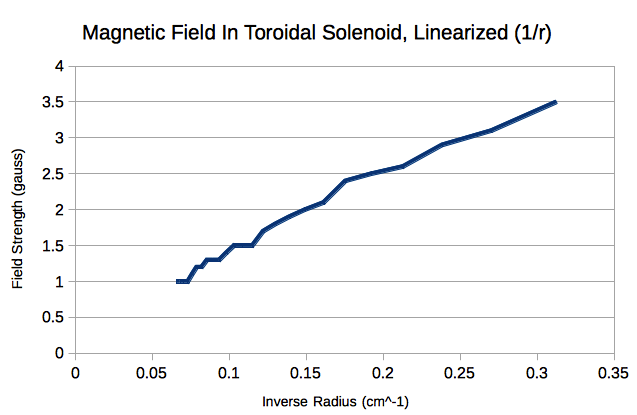
\includegraphics[width=80mm]{toroid_hall_lin.png}
\caption{Measurement of azimuthal magnetic field magnitude in solenoid, plotted
against inverse distance.}
\label{fig:toroid_hall_lin}
\end{figure}

The magnetic field of permanent magnets is unlike that inside a solenoid - the
magnetic flux is not contained, so it must decay more rapidly with the distance
than any infinite amount of current could produce. Indeed, the simplest model
for this would be a dipole, and measurements were taken far enough away from
    the permanent magnets that the magnetic field closely resembles a dipole.
    This means it must follow the proportionality of expression~\ref{dipole}.

\begin{equation}
\label{dipole}
B \propto \frac{1}{r^3}
\end{equation}

The strength of the magnetic field will change depending on the dipole's
relative orientation, but the proportionality should not change. To demonstrate
this in a dipole, measurements of a single component (the z-component) were
taken both above the magnet, moving vertically, and to the side of the magnet,
moving horizontally. It is visible in Figures \ref{fig:maghall_vert_lin} and
\ref{fig:maghall_horiz_lin} that the horizontal magnetic field is weaker, but they
both appear to decay exponentially.
 

\begin{figure}[ht!]
\centering
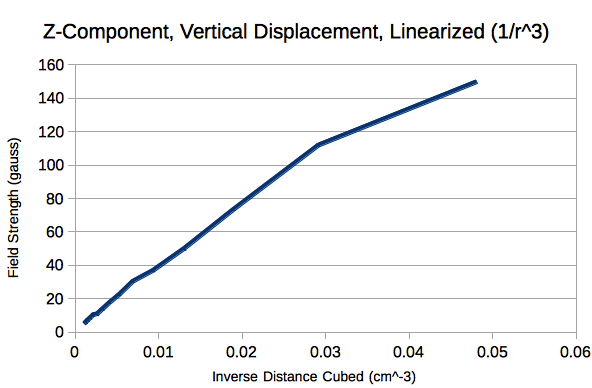
\includegraphics[width=80mm]{maghall_vert_lin.png}
\caption{Measurement of z-component of magnetic field, as a function of
vertical distance from the center, plotted against inverse distance cubed.}
\label{fig:maghall_vert_lin}
\end{figure}

To make the analysis more correct, subsets of the data were chosen such that
the field closely resembled a dipole field, but the data still spanned a wide
range of field strengths. In the vertical case, distances above $4.25 cm$ were
used, with the field strength spanning a range from 5 to 50 gauss. A linear
regression yields a slope of $4044 \pm 79 gauss \cdot cm^3$, with an r value of 0.996
- as good a fit as the toroidal field.

\begin{figure}[ht!]
\centering
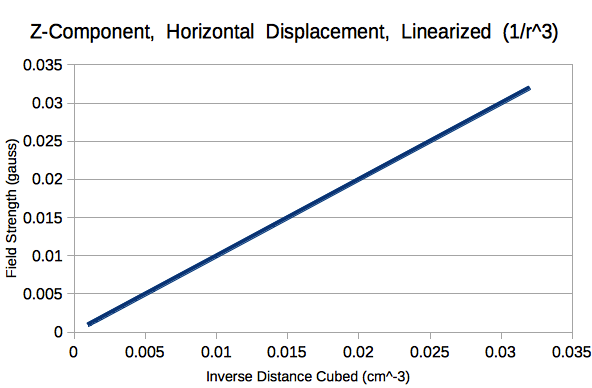
\includegraphics[width=80mm]{maghall_horiz_lin.png}
\caption{Measurement of z-component of magnetic field, as a function of the
horizontal distance to the center, plotted against inverse distance cubed.}
\label{fig:maghall_horiz_lin}
\end{figure}

The horizontal values were similarly chosen. Only data from a distance of $4.15
cm$ was used, spanning a range from 2 to 20 gauss. The field is noticeably
weaker, and the slope is also lower - only $1405 \pm 35 gauss \cdot cm^3$. The r
value is also slightly lower - only 0.991. It would be difficult to improve the
value in this situation, because the field to the side of the magnet is weaker
- selecting a smaller subset of data also means increasing the uncertainty, so
the precision is bounded by the strength of the magnet. However, it still
appears to be a good fit.

The force between magnets is follows another proportionality. It is the
interaction between two dipoles, which means it dies off in strength even
quicker than the magnetic field magnitude of a single magnet. In this case, the
proportionality follows expression \ref{dipole_force}.

\begin{equation}
\label{dipole_force}
B \propto \frac{1}{r^4}
\end{equation}

Using the data in Figure~\ref{fig:magforce_lin}, and performing a regression
analysis after taking the inverse of the distance to the fourth power, a slope
of $28430 \pm 350 g \cdot cm^4$ is obtained. This model has an even higher
r-value, 0.998. This may be because the weight given by the scale is much more
precise than that of the Hall sensor used for previous data sets.

\begin{figure}[ht!]
\centering
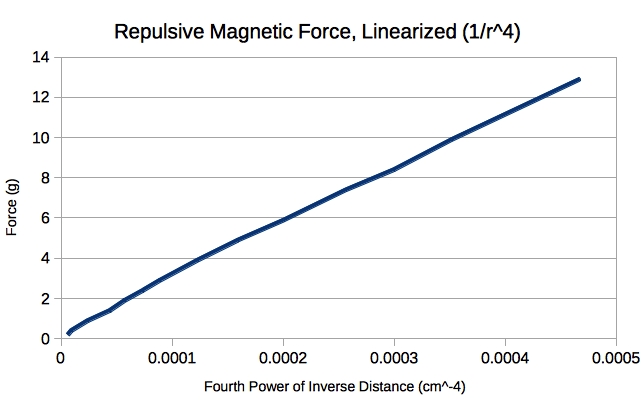
\includegraphics[width=80mm]{magforce_lin.png}
\caption{Measurement of the repulsive force between two magnets, as a function
of center-to-center distance between them, plotted against $r^{-4}$.}
\label{fig:magforce_lin}
\end{figure}

The induced voltage in the solenoid should obey Faraday's law, which states
that the induced current is proportional to the change in magnetic flux inside
the loop (Equation~\ref{faraday}.

\begin{equation}
\label{faraday}
V_{ind} = -\frac{d \Phi_B}{dt}
\end{equation}

If there are N loops, the total voltage induced is simply multiplied by N.

In addition, it is known that the inner loop generates a uniform magnetic field
of

\begin{displaymath}
B = \mu_0 n I_0 sin(\omega t)
\end{displaymath}

inside the surface, of area A. This can be used to calculate the flux, and
substituted into Equation~\ref{faraday} to find the following expression for
the induced voltage.

\begin{displaymath}
V_{ind} = -\frac{d}{dt} \left( \mu_0 n I_0 sin \left( \omega t \right) \cdot A
\right)
\end{displaymath}

Taking the derivative, and ignoring the negative sign (it only signifies a
phase shift).

\begin{equation}
\label{induced_v}
V_{ind} = I_0 \mu_0 \omega A n N cos \left( \omega t \right) = V_0 \left(
\omega t \right)
\end{equation}

Where $V_0$ is the amplitude of the induced voltage. Using the values stated in
the experimental results, in addition to a current amplitude $I_0 = 0.05399 \pm
0.00001 A$ calculated from the differences between the highest and lowest
currents in Figure~\ref{fig:ac_induced}, one obtains a value for $V_0$, shown
in Table 1.

\begin{table}[h]
\centering
\caption{\normalsize{Induced Voltage Amplitudes}}
\scalebox{.9}{
\begin{tabular}{|l|l|}
	\hline
	Measured & Calculated \\ \hline
	$0.021502 \pm 1E-6 V$ & $1.23 \pm 0.06 V$ \\ \hline
	\end{tabular}
}
\medskip
\caption{Table 1: Directly measured induced voltage amplitude, and the
Faraday's law calculation of voltage amplitude}
\end{table}

This is very large difference - enough that percent difference is close to
100\%, because calculated value is off by two orders of magnitude. This could
be explained by a flaw in experimental setup - the assumption of
Equation~\ref{induced_v} is that the entirety of the flux of the inner coil is
located in the outer coil. If the two coils were not aligned correctly, the
flux dies off quickly - with the inverse cube, as was found earlier in the lab
- which would dramatically decrease the induced voltage.

\section{Conclusion}

The fit for generated magnetic fields were all good. The inverse-distance model
for a toroidal solenoid had an r value of 0.996. The inverse-distance-cubed
    models for the field generated by permanent magnets had r values of 0.996
    and 0.991 for the field above and to the side of the magnet respectively -
    the latter possibly smaller because of a decrease in relative precision
    (the field to the side of a dipole is smaller than directly above it). The
    r value for the force between two magnets as the inverse radius to the
    fourth power was by far the best - 0.998, and visual analysis of
    Figure~\ref{fig:magforce_lin} appears nearly perfectly linear.

However, the error in induced voltage calculations was very large - 1.23 V
theoretically vs. 0.02 in reality. This difference is large enough that it is
likely there was a problem with the experimental setup. Specifically, a
misalignment of the inner solenoid and the outer coil. Since the magnetic field
dies off so quickly with a dipole field - which a solenoid generates outside of
itself - a relatively small displacement of the two coils would produce a
dramatic difference in induced voltage. This experiment should be repeated,
with the alignment fixed.
\end{document}


